\documentclass[11pt,a4paper]{article}

\usepackage[utf8]{inputenc}
\usepackage[T1]{fontenc}
\usepackage{lmodern}
\usepackage{amsmath,amssymb,amsthm}
\usepackage{graphicx}
\usepackage{booktabs}
\usepackage{siunitx}
\usepackage{geometry}
\usepackage{caption}
\usepackage{subcaption}
\usepackage[colorlinks=true,linkcolor=blue,citecolor=blue,urlcolor=blue]{hyperref}
\usepackage{xcolor}

\geometry{margin=2.2cm}

% Figure search paths: pick PDFs already mirrored into the Overleaf folder
% and additional PDFs that live under results/.
\graphicspath{{./}{../Overleaf---MFBO-NMPC/}{../results/graphical_results/}{../results/graphics/}{../results/}}

\newcommand{\jtrack}{J_{\mathrm{track}}}
\newcommand{\jtv}{J_{\mathrm{TV}}}
\newcommand{\sse}{\mathrm{SSE}}
\newcommand{\ssdu}{\mathrm{SSdU}}
\newcommand{\Nc}{N_c}
\newcommand{\Np}{N_p}
\newcommand{\Ts}{T_s}
\newcommand{\Cheb}[1]{\mathrm{Cheb}_5\!\left(#1\right)}

\title{Multi-Fidelity Bayesian Optimization for NMPC Tuning:\\
A Documentation and Analysis Report}
\author{Codebase walkthrough of \texttt{MFBO\_NMPC}}
\date{May 2026}

\begin{document}

\maketitle

\begin{abstract}
This report documents the simulation, optimization, and analysis pipeline of the \texttt{MFBO\_NMPC} project. The codebase implements a runtime-aware multi-fidelity Bayesian optimization (MFBO) workflow for bi-objective nonlinear model predictive control (NMPC) tuning on a reduced bioprocess dilution plant. We describe the plant model, the NMPC formulation with an LQR-derived terminal cost, the multi-fidelity closed-loop evaluation policy, the surrogate model used to extrapolate truncated-horizon costs, and the Bayesian-optimization loop that drives the search. We then walk through every root-level script whose name starts with \texttt{main} and every script under \texttt{Result analysis/}, identifying what each one accomplishes and which figures it generates. We provide per-figure discussion of the published artefacts and close with an overall assessment of the optimization behaviour, the surrogate's modelling regime, and the practical implications for controller deployment.
\end{abstract}

\section{Introduction}

NMPC tuning is simulation-expensive: each candidate parameter vector requires a closed-loop simulation that solves a nonlinear program (NLP) at every sampling instant. The cost of such a simulation depends strongly on tuning choices --- longer horizons, tighter weights, harder constraint regimes --- and the objective landscape is non-smooth in a way that defeats gradient-based optimization. The \texttt{MFBO\_NMPC} project addresses this problem with three coupled mechanisms: \textit{(i)} a fidelity variable that truncates the closed-loop simulation horizon to reduce per-evaluation cost; \textit{(ii)} a polynomial fraction surrogate that extrapolates truncated cost to a full-horizon estimate; and \textit{(iii)} a runtime-aware Bayesian-optimization acquisition that explicitly penalizes expensive candidates while still pursuing hypervolume improvement on a bi-objective Pareto front.

The remainder of this document is organized as follows. Section~\ref{sec:methods} formalizes the plant, controller, surrogate, and optimization loop. Section~\ref{sec:mainscripts} catalogues the root-level driver scripts. Section~\ref{sec:analysisscripts} covers the analysis scripts and the figures they produce. Section~\ref{sec:results} provides per-figure discussion of the published artefacts. Section~\ref{sec:discussion} synthesizes the cross-cutting observations and Section~\ref{sec:conclusion} concludes.

\section{Methods}
\label{sec:methods}

\subsection{Plant model}

The plant is a three-state reduced bioprocess dilution model with states $x = [V, X, S]^\top$ (volume, biomass, substrate) and inputs $u = [F_{\mathrm{in},1}, F_{\mathrm{in},2}, F_{\mathrm{out}}]^\top$, governed by
\begin{align}
\dot V &= F_{\mathrm{in},1} + F_{\mathrm{in},2} - F_{\mathrm{out}}, \\
\dot X &= \left(-\frac{F_{\mathrm{in},1}+F_{\mathrm{in},2}}{V} + \mu(S) - k_d\right) X, \\
\dot S &= \frac{(S_{\mathrm{in}}-S)F_{\mathrm{in},1} - S F_{\mathrm{in},2}}{V} - \mu(S)\, X\, Y_{XS}^{-1},
\end{align}
with Monod kinetics $\mu(S) = \mu_{\max}\, S / (K_s + S)$ and parameters $S_{\mathrm{in}} = \SI{70}{g\per L}$, $\mu_{\max} = \SI{0.273}{h^{-1}}$, $K_s = \SI{0.007}{g\per L}$, $k_d = \SI{0.006}{h^{-1}}$, $Y_{XS} = 0.42042$. State and input bounds are $V \in [0.5, 2]$, $X \in [0, 50]$, $S \in [-0.1, 20]$, $u_i \in [0, 0.4]$, $i = 1,2,3$. Plant simulation uses \texttt{ode45} with non-negativity enforcement on $X$ and $S$.

\subsection{NMPC formulation with LQR-derived terminal cost}

At each control step $k$, NMPC solves
\begin{align}
\min_{\{u_{j|k}\}_{j=0}^{\Nc-1}} \quad &
\sum_{j=0}^{\Np-1}\|x_{j|k}-x_{sp}\|_{Q}^2
+ \sum_{j=0}^{\Nc-1}\|u_{j|k}-u_{sp}\|_{R_u}^2 \nonumber\\
&+ \sum_{j=0}^{\Nc-1}\|\Delta u_{j|k}\|_{R_{\Delta u}}^2
+ \left\|\begin{bmatrix} x_{\Np|k}-x_{sp}\\ u_{\Nc-1|k}-u_{sp}\end{bmatrix}\right\|_{P}^2 \\
\text{s.t.}\quad &
x_{0|k}=x_k,\quad x_{j+1|k}=f_{\mathrm{plant}}(x_{j|k},u_{j|k}), \nonumber\\
& x_{j|k}\in\mathcal{X},\quad u_{j|k}\in\mathcal{U}, \nonumber\\
& u_{j|k}=u_{\Nc-1|k},\quad j=\Nc,\ldots,\Np-1, \nonumber
\end{align}
solved with \texttt{fmincon}-SQP on scaled decision variables. Weights are parameterized in base-10 log-scale,
\begin{equation}
Q = \mathrm{diag}(10^{q_1}, 10^{q_2}, 10^{q_3}), \quad
R_u = \mathrm{diag}(10^{r_{u,1}}, 10^{r_{u,2}}, 10^{r_{u,3}}), \quad
R_{\Delta u} = \mathrm{diag}(10^{r_{\Delta u,1}}, 10^{r_{\Delta u,2}}, 10^{r_{\Delta u,3}}).
\end{equation}
In the BO runs driven by \texttt{main.py}, free log-weight exponents are bounded in $[-3,3]$, so the corresponding diagonal entries range from $10^{-3}$ to $10^3$. The first state-weight exponent is fixed at $q_1=0$ in the Python optimization layer, hence $Q_{11}=1$ for the reported BO search even though the MATLAB evaluator itself simply decodes whatever exponent is supplied. This distinction matters because some standalone MATLAB DOE/debug and benchmark configurations use different fixed state weights, for example $Q=\mathrm{diag}(10,1,1)$. The two BO cases also differ in the input penalty: Case~1 pins $r_u=-1000$ so $R_u$ is effectively zero, while Case~2 treats $r_u$ as a free vector in $[-3,3]^3$.
Horizons are encoded as $\Nc = \theta_m + 1$ and $\Np = \theta_p + \Nc$ with integer variables $\theta_p \in [0, 15]$, $\theta_m \in [0, 7]$.

\paragraph{Terminal cost from an offline LQR design.}
The terminal cost matrix $P$ is built offline. Linearizing the plant about its steady-state target yields $(A, B)$, which are discretized in incremental form to $(A_i, B_i)$ at sample time $\Ts = 1/60$~h. A discrete LQR gain $K$ is computed via \texttt{dlqr} using design weights $(Q_{\mathrm{lqr}}, R_{u,\mathrm{lqr}}, R_{\Delta u,\mathrm{lqr}})$ whose log-exponents are obtained by an offline outer optimization (\texttt{TerminalCost/LQR\_tuning.m}) that minimizes the closed-loop integrated squared error plus regularization terms over two representative initial conditions, $x_{0,\mathrm{lqr}}^{(1)} = [1.1, 5, 1]^\top$ (off-volume, low biomass, low substrate; tests start-up tracking) and $x_{0,\mathrm{lqr}}^{(2)} = [1, X_{sp,\mathrm{lqr}}+2, 0]^\top$ with $X_{sp,\mathrm{lqr}} = 15$ (overshoot configuration that tests regulatory recovery from above the biomass setpoint). The resulting LQR tuning vector $\eta_{\mathrm{lqr}} = [-1.998, 0.0003, 1.485, 0.527, -0.974, 0.043, 0.107, -0.118]$ is hard-coded as the design weights used for terminal-cost construction.

Because the NMPC stage weights $(Q, R_u, R_{\Delta u})$ generally differ from the LQR design weights, the terminal cost needs to be computed from the LQR gain matrix $K$ under the new weights. Following standard infinite-horizon-evaluation theory (\texttt{TerminalCost/HowToCompute.m}), $P$ is constructed by solving the discrete Lyapunov equation
\begin{equation}
\label{eq:Plyap}
P = A_{\mathrm{cl}}^\top P\, A_{\mathrm{cl}} + \bar Q, \qquad
\bar Q = S_x^\top Q\, S_x + (S_u - K)^\top R_u (S_u - K) + K^\top R_{\Delta u} K,
\end{equation}
where $A_{\mathrm{cl}}$ is the LQR closed-loop matrix and $S_x, S_u$ are state-/input-selection matrices from the augmented incremental formulation. The function \texttt{construct\_P} (in \texttt{TerminalCost/LQR\_functions/}) implements~\eqref{eq:Plyap} and is called fresh for every candidate $\theta$ because $(Q, R_u, R_{\Delta u})$ vary across the search.

\subsection{Multi-fidelity closed-loop evaluation}

\paragraph{Terminology.}
Throughout this report we distinguish two orthogonal notions that are easily conflated:
\begin{itemize}
    \item \emph{Case 1} / \emph{Case 2} refer to the two independent BO tuning runs that differ in their input-penalty $R_u$ configuration. Specifically, \emph{Case 1} pins the three $r_u$ exponents to $-1000$ in optimization space (so that $R_u = \mathrm{diag}(10^{r_{u,1}}, 10^{r_{u,2}}, 10^{r_{u,3}})$ underflows to the zero matrix and the input penalty is effectively disabled), while \emph{Case 2} releases those exponents and treats $r_u$ as a free optimization variable in $[-3, 3]^3$. Wherever a figure label or numerical summary says ``Case~$i$'', it means the $i$-th BO run.
    \item \emph{Scenario} refers to a simulation setup (initial condition, setpoint trajectory, horizon, noise). Two \emph{simulation scenarios} ($s = 1, 2$) share the same fixed setpoint ($V_{sp} = 1$, $X_{sp} = 20$) and 10~h horizon but use different initial conditions. The first, $x_0^{(1)} = [1.0, 10, 0]^\top$, represents a typical fermentation start: the volume is already at its setpoint, biomass is moderate, and substrate is depleted so that input flow is required for biomass to grow. The second, $x_0^{(2)} = [1.1, 25, 5]^\top$, is designed to keep $F_{\mathrm{in},2}$ ($u_2$) from collapsing to zero while its associated $R_u$ and $R_{\Delta u}$ increases to their upper bound; it tests regulatory action that must approach the setpoint from above and compensate biomass overshoot. Both scenarios are evaluated inside every BO query. A separate \emph{validation scenario} is the 30~h three-step setpoint schedule $X_{sp}: 7 \to 13 \to 16$ used in Section~\ref{sec:results} to test transferability.
\end{itemize}

Each candidate $\theta = [f, \theta_p, \theta_m, q, r_u, r_{\Delta u}] \in \mathbb{R}^{12}$ is evaluated by simulating both simulation scenarios $s \in \{1, 2\}$ over a fidelity-dependent horizon
\begin{equation}
t_f(f) = 10 f \;\mathrm{h}, \qquad N(f) = \left\lceil t_f(f)/\Ts \right\rceil + 1, \qquad f \in [0.01, 1].
\end{equation}
The truncated-horizon bi-objective is defined by summing across both simulation scenarios,
\begin{align}
\jtrack^{\mathrm{part}}(\theta, f) = \sse^{\mathrm{part}}(\theta, f) &= \sum_{s=1}^2 \sum_{k=0}^{N(f)-1} \left\| (x_{k,s} - x_{sp}) \odot [10, 1, 1]\right\|_2^2, \\
\jtv^{\mathrm{part}}(\theta, f) =  \ssdu^{\mathrm{part}}(\theta, f) &= \sum_{s=1}^2\sum_{k=1}^{N(f)-1} \|u_{k,s} - u_{k-1,s}\|_2^2,
\end{align}

The full-horizon estimates used by BO follow from a single Chebyshev fraction model per objective,
\begin{equation}
\jtrack(\theta, f) = \frac{\jtrack^{\mathrm{part}}(\theta, f)}{\phi_{\sse}(f)},
\qquad
\jtv(\theta, f) = \frac{\jtv^{\mathrm{part}}(\theta, f)}{\phi_{\ssdu}(f)},
\end{equation}
with $\phi_i(f) = \mathrm{clip}\!\left(\Cheb{2f-1; c_i}, 0.01, 1\right)$ for $i \in \{\sse, \ssdu\}$. The fixed Chebyshev coefficients (six values per objective) are fitted offline in \texttt{J~surrogate/surrogate.m} on normalized cumulative trajectories, achieving $R^2 = 0.9998$ for $\sse$ and $R^2 = 0.9919$ for $\ssdu$.

\subsection{Bayesian-optimization setup}

The optimization is cast as maximization of $y(\theta) = -[\jtrack(\theta), \jtv(\theta)]^\top$. Two Gaussian-process models are fit at every iteration: $\mathcal{M}_{\mathrm{obj}}: \theta \mapsto y(\theta)$ and $\mathcal{M}_{\log t}: \theta \mapsto \log t(\theta)$, both using \texttt{SingleTaskGP} with input normalization and output standardization. The acquisition is a log-domain composition of \texttt{qLogNoisyExpectedHypervolumeImprovement} (qLogNEHVI) with a fidelity-bias term and a runtime penalty,
\begin{align}
\log \alpha(\theta) &= \log \texttt{qLogNEHVI}(\theta) + w_z \log(a_z(f) + \varepsilon) - w_t \gamma \log(\mathbb{E}[t(\theta)] + \varepsilon),\\
a_z(f) &= \exp\!\left(-\frac{(1-f)^2}{2 \ell_z^2}\right), \qquad
\mathbb{E}[t(\theta)] = \exp\!\left(\mu_{\log t}(\theta) + \tfrac{1}{2}\sigma^2_{\log t}(\theta)\right),
\end{align}
with $\ell_z = 0.25$, $\gamma = 1$, $w_z = w_t = 1$, $\varepsilon = 10^{-6}$, and $\mathbb{E}[t]$ lower-bounded by the best observed runtime. Reference points for the hypervolume calculation are updated from data as $r_j = y_{j,\min} - 0.2(y_{j,\max} - y_{j,\min})$. Each run uses $N_{\mathrm{init}} = 20$ scrambled-Sobol design-of-experiment (DOE) points followed by 101 optimization iterations (121 evaluations total). Two runs are reported under identical settings to expose path dependence.

\subsection{Software organization}

The codebase is organized into two layers. Root-level \texttt{main*} scripts drive every kind of NMPC simulation needed (live MFBO loop, fixed Pareto replays, fixed-benchmark controllers, setpoint-schedule comparison). The \texttt{Result analysis/} folder transforms simulation artefacts into figures and tables for the manuscript. A single orchestrator, \texttt{Result analysis/run\_analysis.m}, regenerates the entire figure set in one invocation.

\section{Root-level driver scripts}
\label{sec:mainscripts}

\subsection{\texttt{main.py}}
The Python side of the MFBO loop. It builds a scrambled-Sobol DOE in optimization space, then iterates by fitting the two GPs, forming the qLogNEHVI acquisition wrapped in a custom \texttt{MFMOLogAcq} class that adds the fidelity bias $w_z \log a_z(f)$ and the runtime penalty $-w_t \gamma \log \mathbb{E}[t]$. Communication with MATLAB is via file I/O: $\theta$ is written to \texttt{inbox/theta.txt}, the worker writes new rows to \texttt{results/results.csv}, and Python logs each evaluation plus acquisition diagnostics to \texttt{results/opt\_trace.csv}. Integer dimensions are rounded after acquisition. Three input-weight dimensions are pinned to $-1000$ so that $10^{r_u}$ underflows to zero, disabling the input penalty as a design choice.

\subsection{\texttt{main\_BO.m}}
The MATLAB-side canonical evaluator. It initializes a \texttt{base} struct once (plant, setpoints, LQR data, fixed noise realization, Chebyshev coefficients) and runs in one of three modes: \texttt{external} (polls \texttt{inbox/theta.txt}), \texttt{doe} (sweeps a predefined matrix), or \texttt{single} (one hard-coded $\theta$ for debugging). The shared evaluator \texttt{simulate\_nmpc} runs the closed loop on both simulation scenarios for $t_f = 10f$ h, then divides the truncated SSE/SSdU sums by $\phi_i(f)$ (floored at $0.01$). Each $\theta$ produces one row in \texttt{results.csv} and one \texttt{.mat} payload.

\subsection{\texttt{main\_NMPC\_test\_runs.m}}
Replays a hand-picked list of Pareto-optimal controllers at full fidelity ($f=1$) and zero noise. Output trajectories are written to \texttt{results/test\_run/\textless run\textgreater \_full\_f1\_no\_noise/}. Downstream consumers: \texttt{analyze\_test\_run\_metrics.m}.

\subsection{\texttt{main\_benchmark\_fix.m}}
Runs a fixed reference NMPC ($m=6$, $p=61$, $Q = \mathrm{diag}(10, 1, 1)$, $R_u = 0$, $R_{\Delta u} = \mathrm{diag}(10, 10, 10)$, $P = 0$) at $f = 1$ both noise-free and with the same-noise realization used during BO. This is the baseline against which Pareto controllers are compared.

\subsection{\texttt{main\_benchmark\_reference\_controller.m}}
Identical to \texttt{main\_benchmark\_fix.m} but retains the default input penalty $R_u = \mathrm{diag}(2, 2, 1)$ from \texttt{NMPC\_terminal}. Provides a controlled comparison isolating the effect of $R_u$.

\subsection{\texttt{main\_final\_fidelity.m}}
Replays all non-DOE Pareto-frontier controllers at $f = 1$ with the same noise realization as BO. This is the ``refined'' evaluation set used to validate whether BO's surrogate-extrapolation ranking matches the true full-horizon ranking.

\subsection{\texttt{main\_setpoint\_schedule\_controller\_comparison.m}}
Simulates each Pareto-selected controller plus the benchmark on a 30~h setpoint-schedule scenario where the biomass target $X_{sp}$ steps through $7 \to 13 \to 16$ at $t = 10, 20$~h. Non-benchmark controllers rebuild $P$ at each setpoint change via the workflow in~\eqref{eq:Plyap}; the benchmark keeps $P = 0$. Evaluates transferability of the BO-tuned set to a regime never seen during optimization.

\section{Analysis scripts}
\label{sec:analysisscripts}

\subsection{\texttt{main\_pareto.m}}
Post-processing hub. Loads \texttt{results.csv} from each run, enforces the policy that DOE iterations $1$--$20$ are excluded from any Pareto/optimization conclusion, computes the non-dominated mask in $(\sse, \ssdu)$ space, summarises runtime by phase, and produces publication-ready figures plus numerical tables. Generates \texttt{pareto\_samples\_run1\_run2.pdf}, \texttt{sse\_vs\_ssdu\_side\_by\_side\_z.pdf}, \texttt{runtime\_vs\_iteration\_side\_by\_side.pdf}, \texttt{runtime\_cumulative\_run1\_run2.pdf}, and \texttt{refined\_frontier\_change.pdf}. Numerical outputs include \texttt{resultssandbox\_runtime\_and\_params.txt} and \texttt{final\_pareto\_frontier\_f1\_noisy\_noiseless\_metrics.csv}.

\subsection{\texttt{resultssandbox.m}}
Predecessor of \texttt{main\_pareto.m}. Produces the same first four PDFs and the same runtime summary, but omits the refined-frontier comparison and the noisy/noiseless metrics export. Useful as a lighter standalone entry point.

\subsection{\texttt{analyze\_test\_run\_metrics.m}}
Computes settling-time, final-error, and IAE diagnostics from the noise-free full-horizon replays. Settling for state $i$ is defined as the earliest time at which $|e_i|/|r_i| \le 5\%$ for all subsequent samples; NaN indicates the final relative error exceeds tolerance. Exports the controller-by-scenario table consumed by \texttt{recover\_boxplot\_data.py}. Numerical outputs: \texttt{analyze\_test\_run\_metrics\_summary.txt}, \texttt{final\_pareto\_counts\_by\_case.txt}, and the boxplot CSVs.

\subsection{\texttt{recover\_boxplot\_data.py}}
Reads the boxplot CSVs and rebuilds the publication-quality figures \texttt{python\_settling\_time\_boxplot.pdf}, \texttt{python\_np\_by\_case\_boxplot.pdf}, and \texttt{python\_nc\_by\_case\_boxplot.pdf}, using the Wong (2011) Nature Methods palette and a horizontal reference at $t = \SI{8.09603}{h}$ corresponding to the combined mean optimization-phase fidelity $z \cdot T$.

\subsection{\texttt{analyze\_setpoint\_schedule\_metrics.m}}
Loads every \texttt{out\_schedule\_*.mat} from the validation scenario, computes per-scenario SSE/SSdU/IAE/settling totals (one entry per tuning-scenario initial condition), builds the 2-objective Pareto subset, and produces both trajectory plots and modified-versus-unmodified boxplots. Generates the manuscript-named PDFs \texttt{results/setpoint\_tracking.pdf} and \texttt{results/setpoint\_tracking\_MV.pdf} alongside the \texttt{results/graphics/setpoint\_schedule\_*} variants. Numerical output: \texttt{setpoint\_schedule\_metrics\_same\_noise.csv}.

\paragraph{Selection of the deployment controller.}
The script identifies candidates programmatically and then commits to one by hand. First, it computes the 2-objective Pareto set on the schedule scenario using $(\sse_{\mathrm{total}}, \ssdu_{\mathrm{total}})$. Second, it restricts to non-benchmark Pareto candidates, computes $\sse_{\mathrm{total}}$ relative to the benchmark, sorts ascending, and keeps the top three as \texttt{coloredControllerIds}. Third, one of those candidates is hard-coded as the deployment pick (\texttt{blackControllerId = "ts\_20260211\_122653\_modified"}). The documented selection rationale: against the benchmark, this controller achieves $16.6\times$ faster wall time (6.02\% of the benchmark's), a $4.49\times$ smaller volume tracking error, an 8.87\% lower SSdU, and biomass IAE within 2\%, at a cost of 11.54\% worse substrate tracking. Two commented-out alternatives (\texttt{ts\_20260210\_180826\_modified} and \texttt{ts\_20260210\_151703\_modified}) each beat the benchmark on subsets of these metrics but lose on others, typically trading substrate quality for volume quality. The selection is therefore a deliberate multi-criteria engineering pick rather than a single-objective optimum.

\subsection{\texttt{plot\_refined\_frontier\_change.m}}
Directly compares the optimization Pareto frontier (after DOE exclusion) against the refined frontier obtained by re-evaluating the same controllers at $f = 1$ with the same noise. Generates \texttt{refined\_frontier\_change.pdf} and the textual report \texttt{results/txt results/refined\_promoted\_frontier\_z\_lt\_1.txt}.

\subsection{\texttt{exploring\_u.m}}
Post-hoc input smoothing experiment for the selected controller. Inputs are partitioned at nodes every $\approx \SI{0.1}{h}$. For each interval between consecutive nodes and each input channel, a linear program enforces the cumulative-sum constraint $\sum_i u^\star_i = \sum_i u_i$ while minimizing $\sum_i |u^\star_i - u^\star_{i-1}|$. Generates \texttt{exploring\_u\_selected\_controller\_same\_noise.pdf}.

\subsection{\texttt{run\_analysis.m}}
Orchestrator. Runs \texttt{analyze\_test\_run\_metrics.m}, then \texttt{recover\_boxplot\_data.py}, then \texttt{main\_pareto.m}, then \texttt{J~surrogate/surrogate.m}, then \texttt{results/numerical~results/compile\_results\_txt.m}, and finally copies every PDF in \texttt{results/graphical\_results/} into \texttt{Overleaf---MFBO-NMPC/}.

\section{Results: per-figure discussion}
\label{sec:results}

\subsection{Pareto structure}

\begin{figure}[!h]
\centering
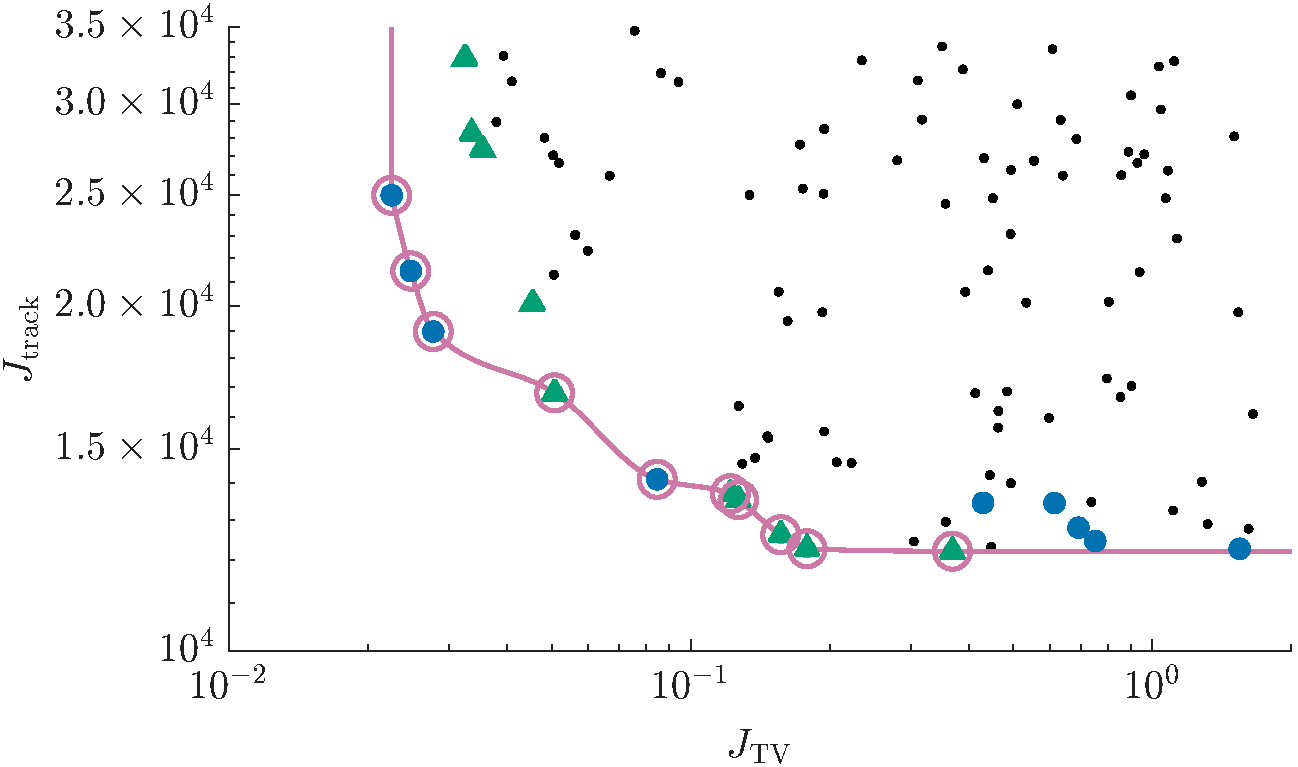
\includegraphics[width=0.9\linewidth]{pareto_samples_run1_run2.pdf}
\caption{Evaluated samples in $(\jtv, \jtrack)$ space and Pareto-optimal points across both BO runs. Each point is one BO evaluation aggregated across the two simulation scenarios. Small black filled dots are all evaluated optimization samples from both runs pooled together. Blue filled circles mark the within-case non-dominated points of Case~1 ($R_u$ pinned to zero), and vermillion filled triangles mark the within-case non-dominated points of Case~2 ($R_u$ as a free variable). Large open orange circles highlight the combined non-dominated frontier obtained when the two runs are merged into a single pool.}
\label{fig:pareto}
\end{figure}

Figure~\ref{fig:pareto} shows a well-defined non-dominated frontier in both runs with a pronounced knee where further reduction in $\jtrack$ requires disproportionately larger $\jtv$. The overlap between the two runs in the knee region is the principal evidence that this compromise is structurally robust for the tested plant and disturbance realization.

A second observation is that the two runs specialize on different segments of the front. Case~1 populates the low-$\jtv$ tail ($\jtv$ down to $0.026$ but $\jtrack$ up to $22{,}781$), while Case~2 populates the low-$\jtrack$ region ($\jtrack$ as low as $12{,}221$ with $\jtv \in [0.13, 0.39]$). Both runs concentrate at $\Nc = 1$, but Case~1's Pareto subset frequently also picks $\Np = 1$ (5 of 9 candidates), whereas Case~2 picks $\Np = 1$ in only 4 of 10. When $\Nc = \Np = 1$, the NMPC optimization horizon collapses to one stage cost plus the terminal $P$, so the resulting policy reduces to the LQR feedback law that built $P$ applied to the nonlinear model at the current state --- a smooth, conservative controller (low $\jtv$) that converges slowly (higher $\jtrack$). When $\Nc = 1$ but $\Np > 1$, a single control move is committed but evaluated against an $\Np$-step prediction of free-state evolution under that move, closed off by the same terminal $P$. This makes the controller more anticipatory, lowering $\jtrack$ at the cost of larger move-to-move corrections. The apparent ``different degrees of freedom'' between the two runs is therefore the same $\Nc = 1$ regime exploring two different sub-modes, with BO's finite-budget path dependence pushing each run into a different sub-mode.

\paragraph{Benchmark comparison.}
The fixed-benchmark replay at $f = 1$ with the same noise realization used during BO, aggregated across both simulation scenarios, gives $\sse \approx 12{,}260$ with $\ssdu \approx 3.52$. The top Case~2 Pareto controllers achieve essentially identical tracking ($\sse \approx 12{,}221$--$12{,}299$) with $\ssdu \in [0.16, 0.39]$ --- roughly $8$ to $22\times$ less control variation. The benchmark therefore sits strictly inside the BO-found Pareto set on this plant: it is excessively aggressive on input movement without an offsetting tracking advantage.

\subsection{Runtime behaviour}

\begin{figure}[!h]
\centering
\begin{subfigure}{0.49\linewidth}
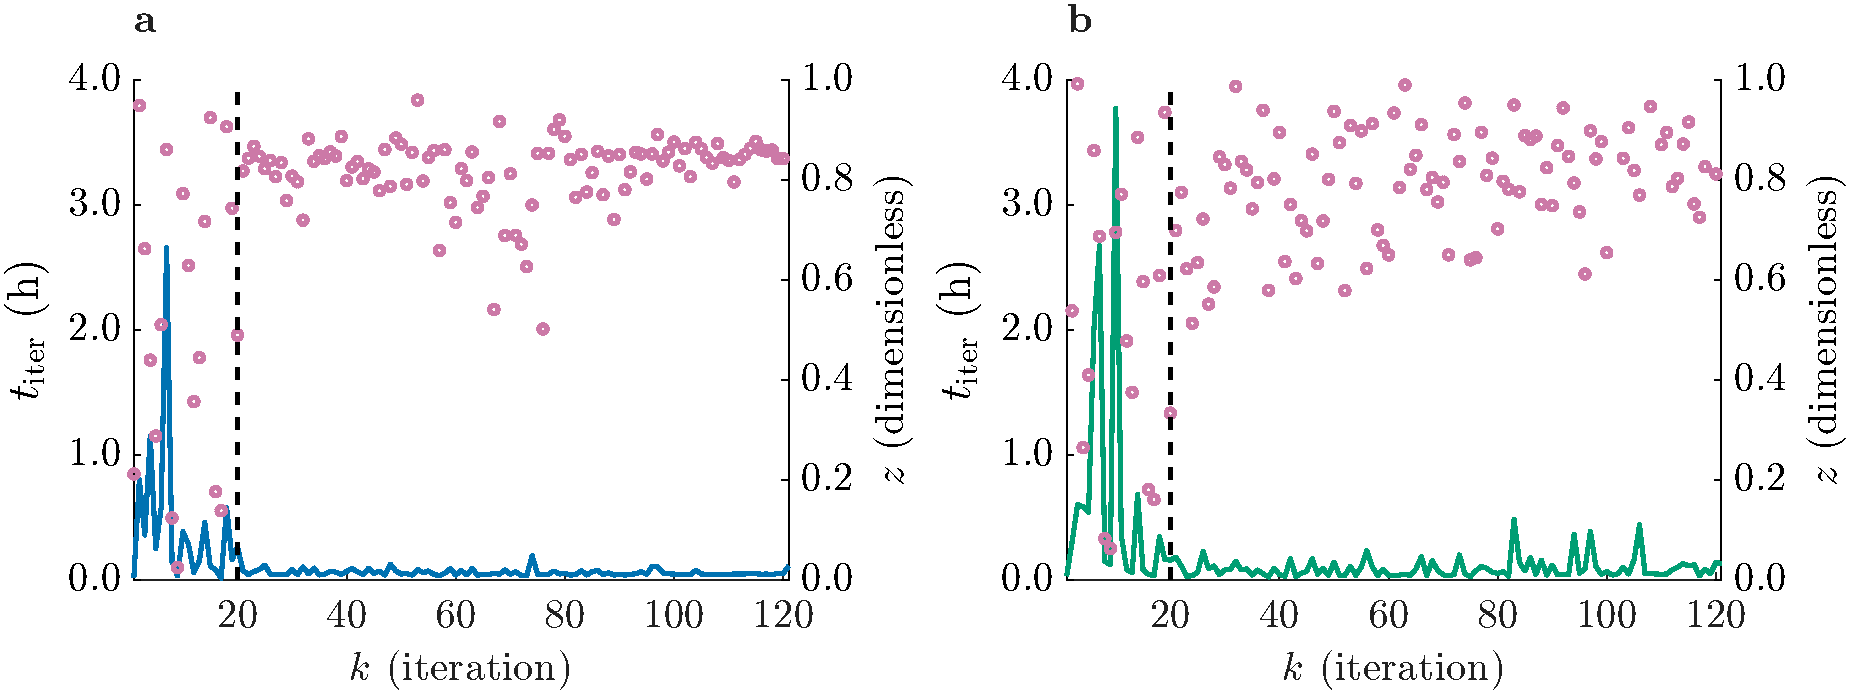
\includegraphics[width=\linewidth]{runtime_vs_iteration_side_by_side.pdf}
\caption{Per-evaluation runtime over iteration. Left subpanel: Case~1 (BO run with $R_u = 0$). Right subpanel: Case~2 (BO run with $R_u$ as a free variable). The shaded region in each subpanel highlights the 20 DOE iterations preceding the optimization phase.}
\label{fig:runtime_iter}
\end{subfigure}
\hfill
\begin{subfigure}{0.49\linewidth}
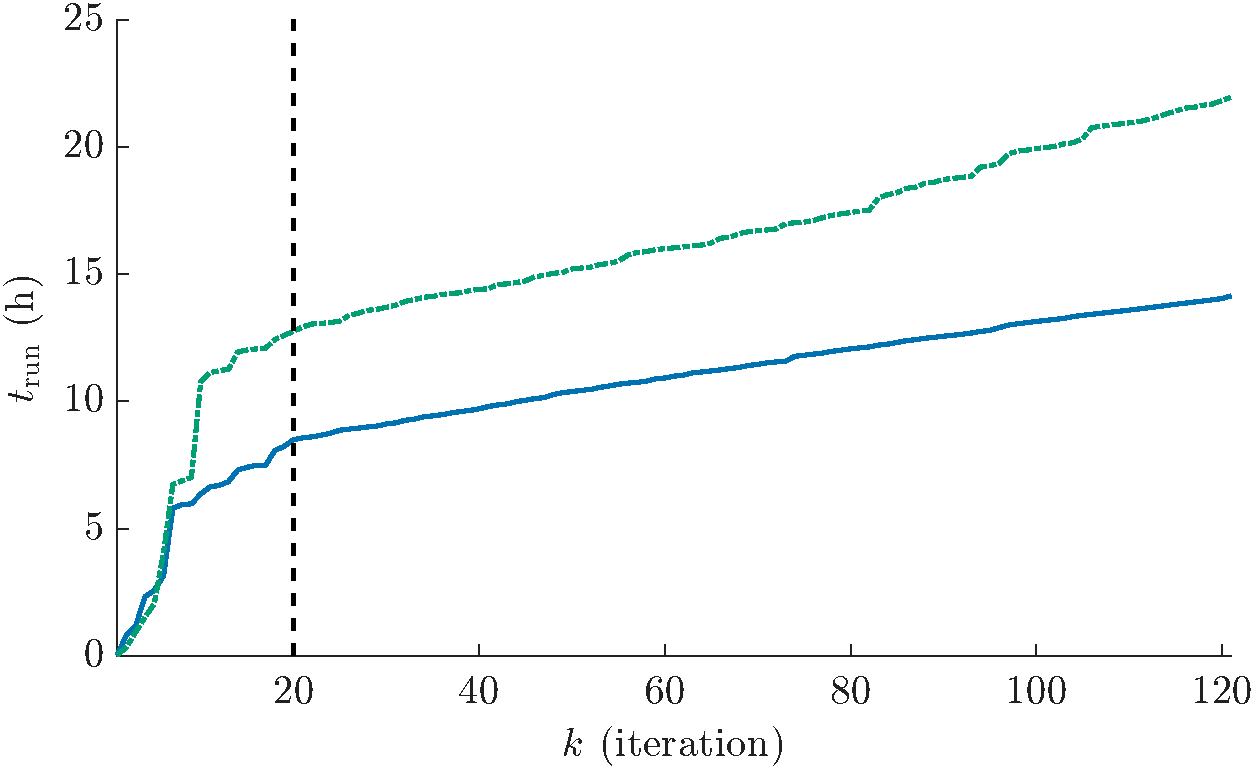
\includegraphics[width=\linewidth]{runtime_cumulative_run1_run2.pdf}
\caption{Cumulative wall-clock runtime. The blue curve is Case~1 ($R_u = 0$) and the vermillion curve is Case~2 ($R_u$ free).}
\label{fig:runtime_cum}
\end{subfigure}
\caption{Runtime allocation across DOE and optimization phases for both BO runs.}
\label{fig:runtime}
\end{figure}

Figure~\ref{fig:runtime} confirms that DOE dominates computational cost in both runs. Case~1 spends 509.69~min in DOE (60.03\%) and 339.36~min in optimization (39.97\%), for a total of 849.05~min. Case~2 spends 765.23~min in DOE (58.08\%) and 552.21~min in optimization (41.92\%), for a total of 1{,}317.44~min. Combined across runs, 1{,}274.92~min of 2{,}166.49~min (58.85\%) are spent in DOE. Average per-evaluation runtime drops from 31.87~min during DOE to 4.41~min during optimization, confirming that the runtime-aware acquisition shifts the search toward cheaper candidates after model initialization. Crucially, the mean optimization-phase fidelity remains high (0.819 in Case~1, 0.800 in Case~2, combined 0.810), so the runtime savings are not produced by collapsing to persistently low fidelity.

\subsection{Fidelity-coloured objective scatter}

\begin{figure}[!h]
\centering
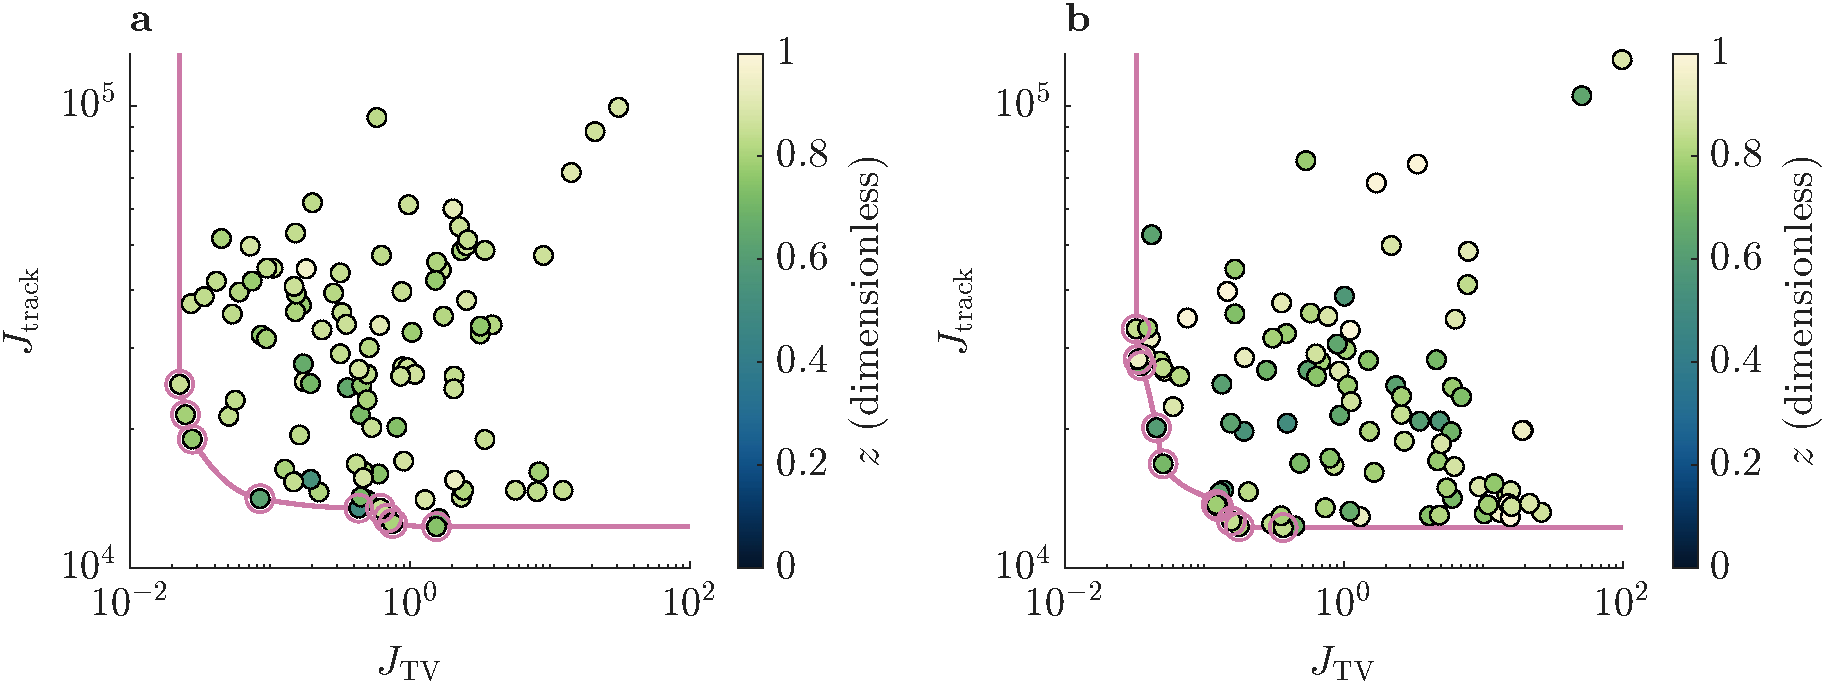
\includegraphics[width=0.95\linewidth]{sse_vs_ssdu_side_by_side_z.pdf}
\caption{Objective space $(\jtv, \jtrack)$ side by side, points coloured by fidelity $z = f$.}
\label{fig:obj_z}
\end{figure}

Figure~\ref{fig:obj_z} resolves the question of \emph{where} the multi-fidelity mechanism concentrates effort. Low-$z$ points spread broadly over exploratory regions of objective space, whereas high-$z$ points cluster near the non-dominated neighbourhoods. This is the intended mechanism: cheap evaluations map global geometry, and expensive evaluations are concentrated where final Pareto quality is determined.

\subsection{Horizon-selection diagnostics}

\begin{figure}[!h]
\centering
\begin{subfigure}{0.49\linewidth}
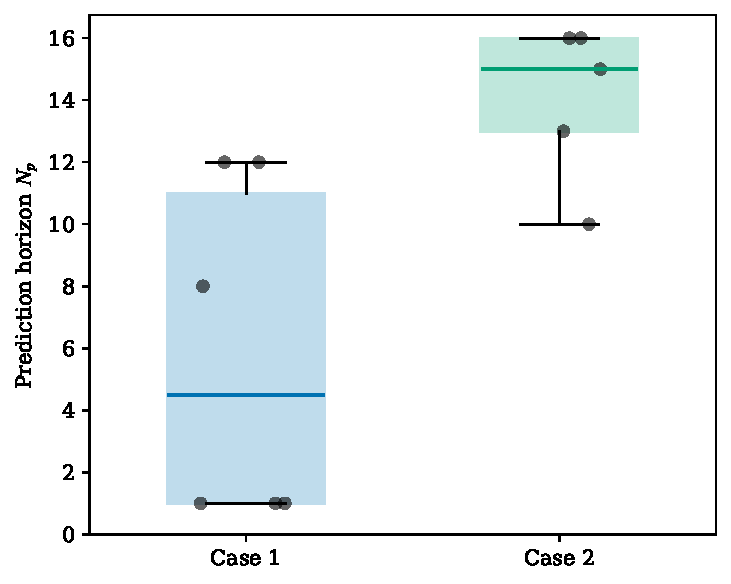
\includegraphics[width=\linewidth]{python_np_by_case_boxplot.pdf}
\caption{Prediction horizon $\Np$ distribution.}
\label{fig:np}
\end{subfigure}
\hfill
\begin{subfigure}{0.49\linewidth}
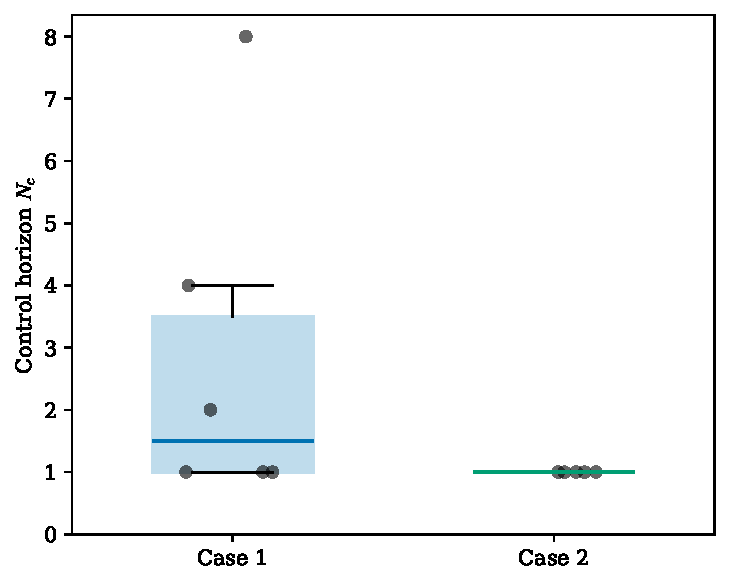
\includegraphics[width=\linewidth]{python_nc_by_case_boxplot.pdf}
\caption{Control horizon $\Nc$ distribution.}
\label{fig:nc}
\end{subfigure}
\caption{Horizon distributions among Pareto-optimal candidates by run.}
\label{fig:horizon}
\end{figure}

Figure~\ref{fig:horizon} reinforces the Section~5.1 observation about horizon selection. Both runs collapse to $\Nc = 1$ among Pareto candidates ($9/9$ in Case~1, $10/10$ in Case~2). $\Np$ is more variable: Case~2 picks larger values than Case~1 in the Pareto set, consistent with Case~2 living at the low-$\jtrack$ end of the front (which rewards prediction-horizon length) and Case~1 living at the low-$\jtv$ end (which favours the LQR-collapsed $\Nc = \Np = 1$ mode).

\subsection{Settling-time diagnostics}

\begin{figure}[!h]
\centering
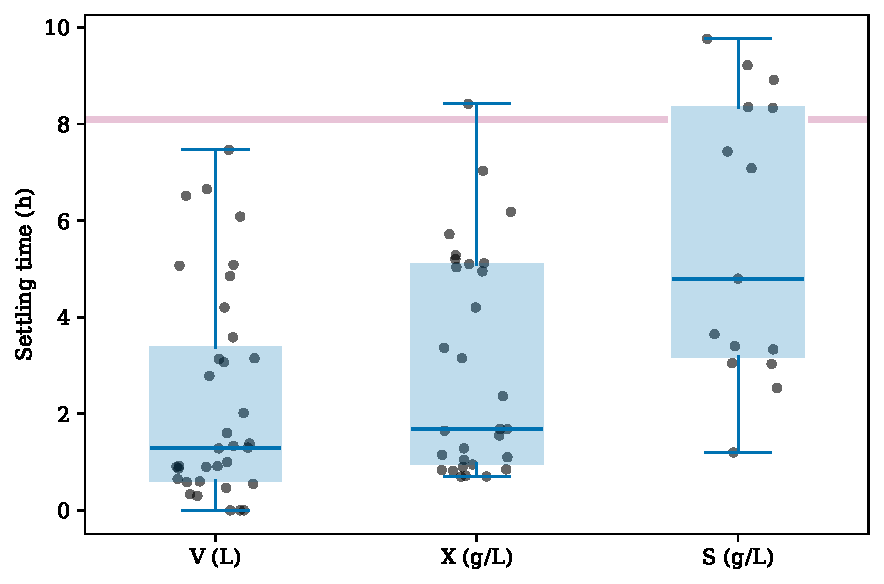
\includegraphics[width=0.7\linewidth]{python_settling_time_boxplot.pdf}
\caption{Settling time distributions at $z = 1$ without noise. The horizontal reference line at $\SI{8.09603}{h}$ corresponds to $z \cdot T$ where $z = 0.81$ is the combined mean optimization-phase fidelity and $T = \SI{10}{h}$ is the full horizon.}
\label{fig:settling}
\end{figure}

Figure~\ref{fig:settling} reveals a strong state-dependent asymmetry. The fraction of runs with NaN settling times (final error above 5\%) is 12.50\% for state~1, 25.00\% for state~2, and 62.50\% for state~3. Using the $\SI{8.09603}{h}$ threshold, settling success is 87.50\% (35/40) for state~1, 72.50\% (29/40) for state~2, and 25.00\% (10/40) for state~3; simultaneous settling of all states is 25.00\% (10/40).

The horizontal reference line at $z \cdot T = \SI{8.096}{h}$ carries an important secondary interpretation. State~1 mostly settles \emph{before} this line, state~2 straddles it, and state~3 mostly does not settle. The fact that BO's mean optimization-phase fidelity $z \approx 0.81$ coincides with the empirical settling timescale of the system is consistent with the runtime-aware acquisition having discovered an empirical truncation horizon that matches the system's natural settling time: past that point, additional simulation samples accumulate near-zero residual error and contribute little new ranking information.

The principal control conclusion is that minimizing $(\jtrack, \jtv)$ does not guarantee balanced state-wise settling, especially for substrate ($S$). This is a modelling choice in the current bi-objective formulation rather than a failure of BO itself.

\subsection{Surrogate diagnostics}

\begin{figure}[!h]
\centering
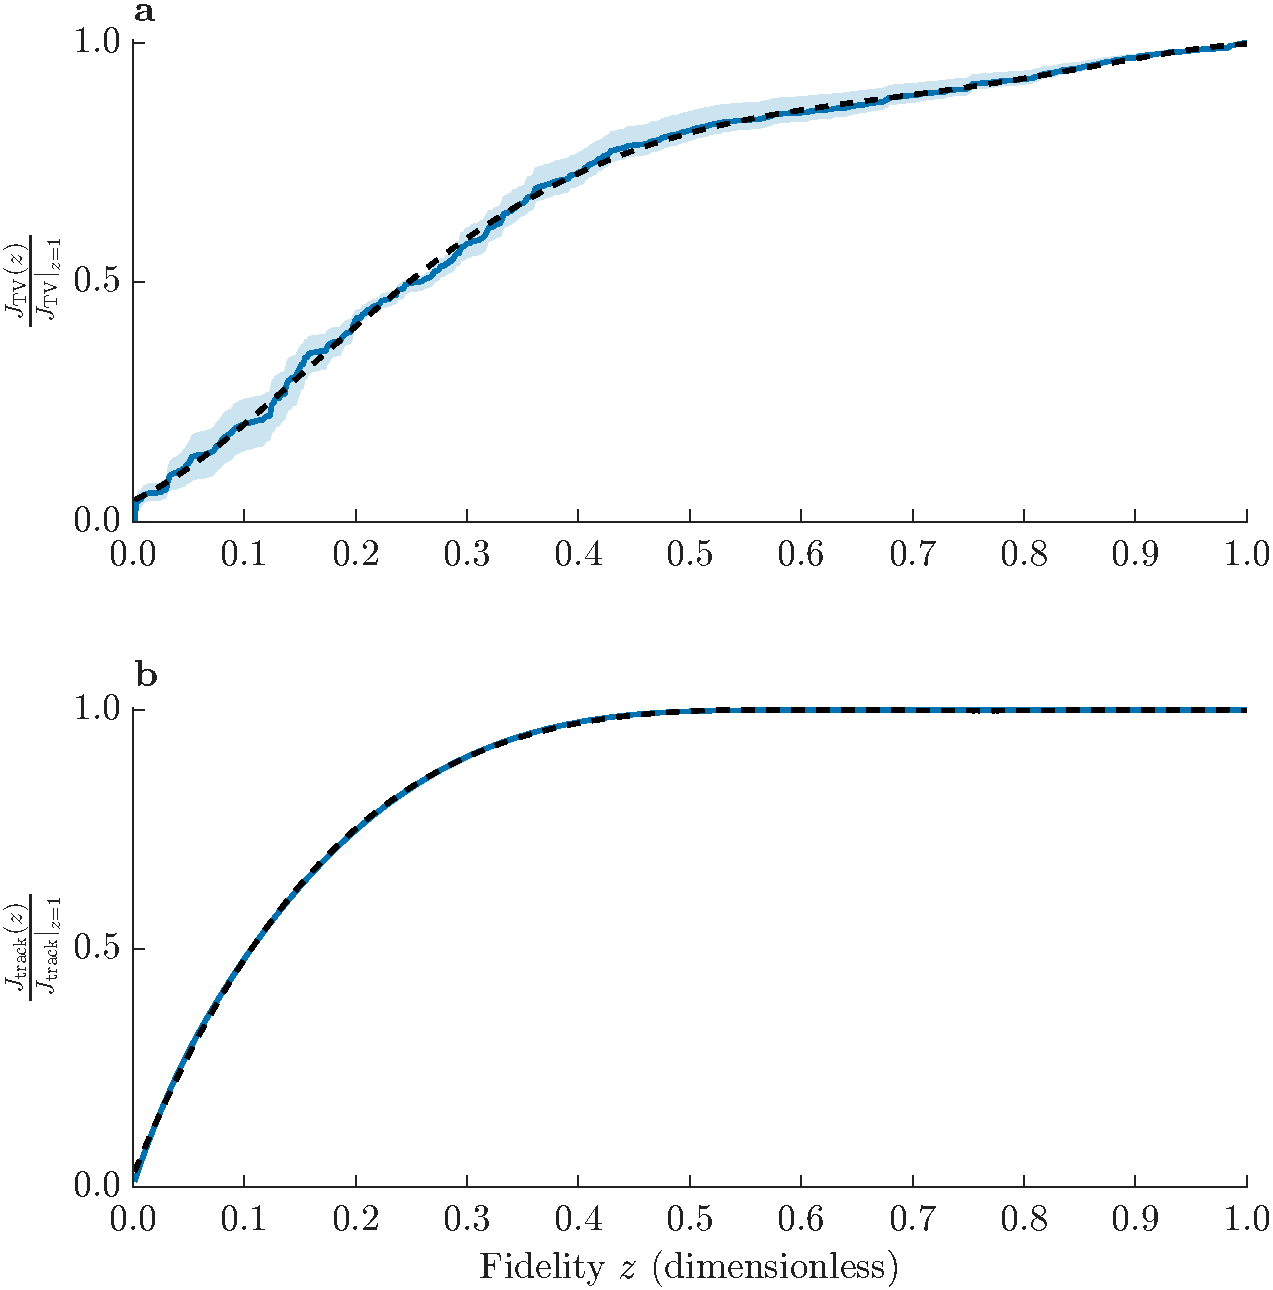
\includegraphics[width=0.7\linewidth]{surrogate_diagnostics_stacked.pdf}
\caption{Aggregated surrogate-fit diagnostics: min--max envelope (shaded), empirical mean trajectory (solid), and fitted Chebyshev curve (dashed) for normalized cumulative $\jtv$ and $\jtrack$ versus fidelity $z$.}
\label{fig:surr_fit}
\end{figure}

\begin{figure}[!h]
\centering
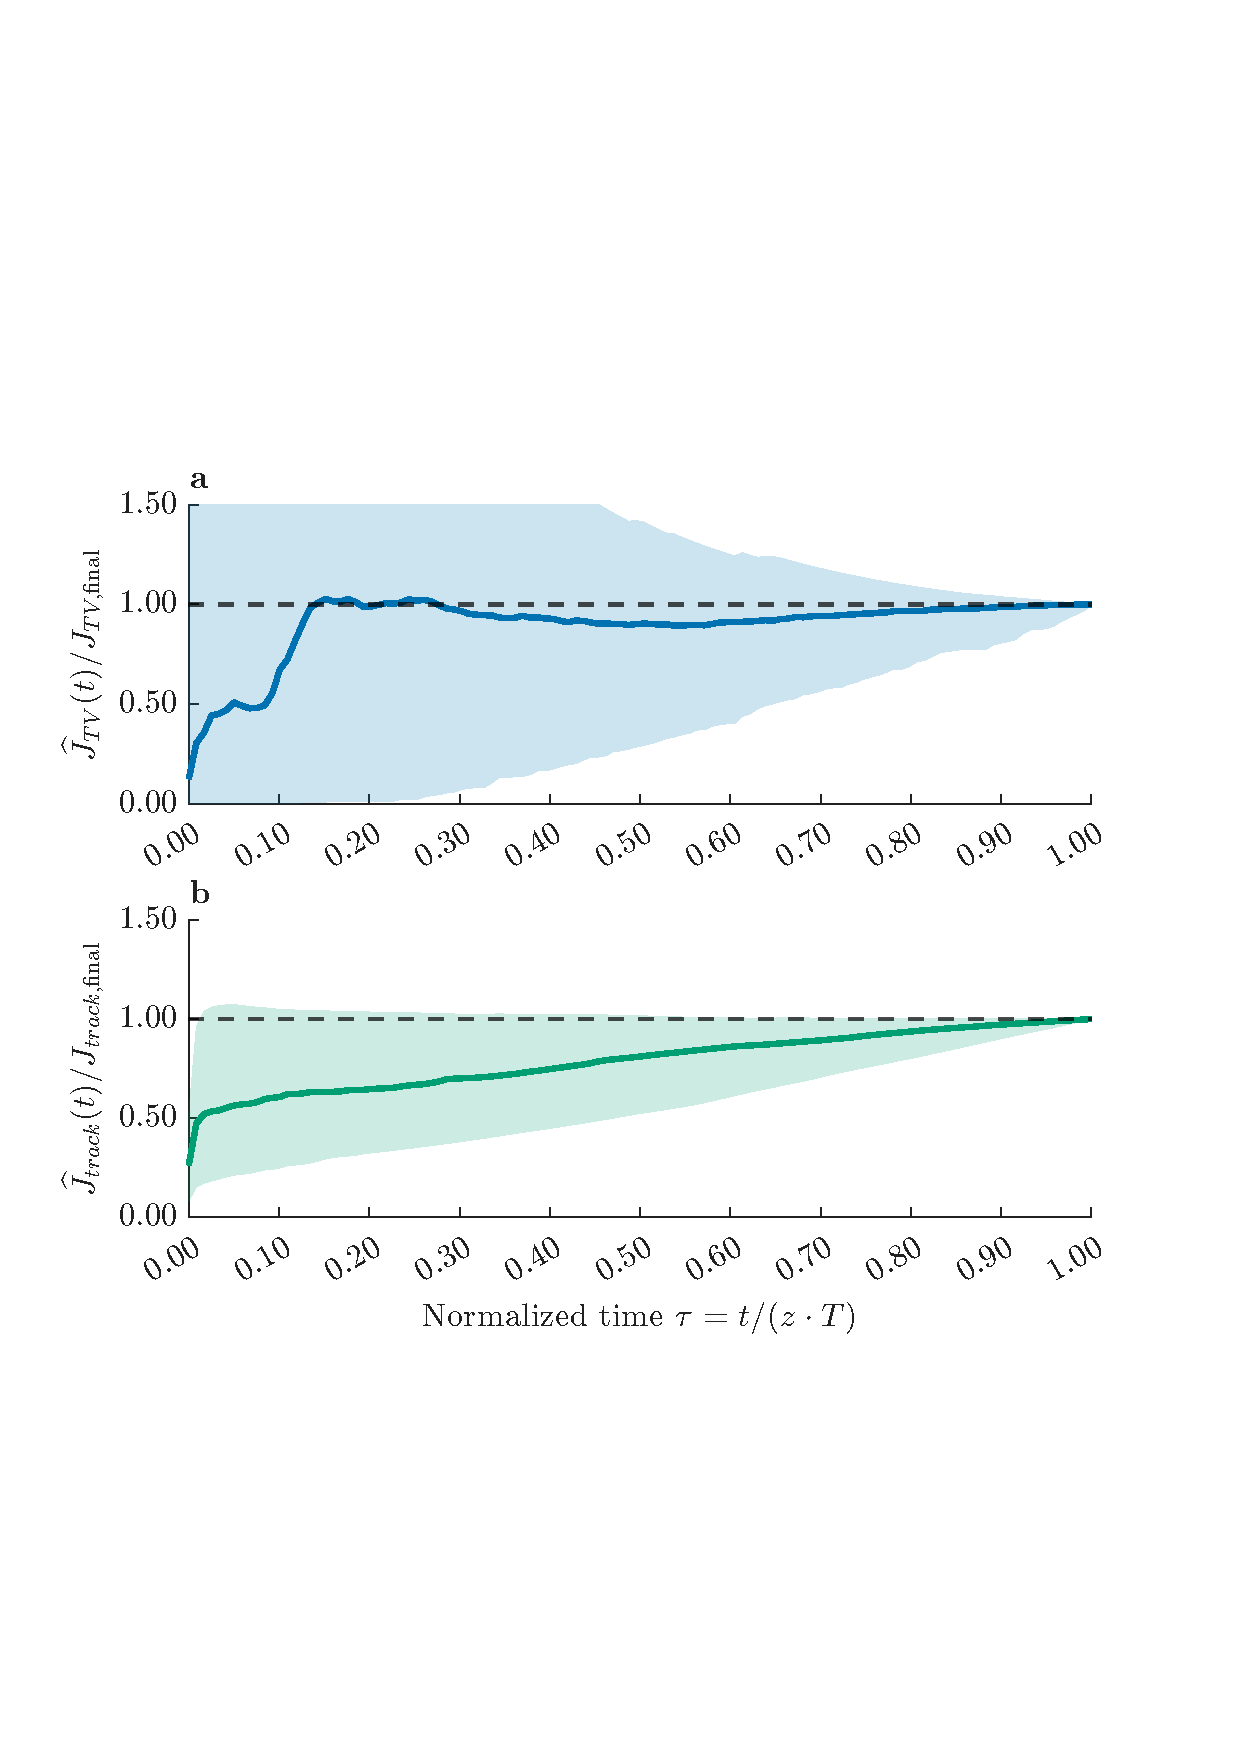
\includegraphics[width=0.7\linewidth]{surrogate_test_ratio_vs_time_95band.pdf}
\caption{Pointwise 95\% empirical quantile envelope for normalized extrapolated trajectories $\widehat\jtv(t)/{\jtv}_{,\mathrm{final}}$ (top) and $\widehat\jtrack(t)/{\jtrack}_{,\mathrm{final}}$ (bottom) across all processed outputs.}
\label{fig:surr_95}
\end{figure}

Figure~\ref{fig:surr_fit} evaluates the offline Chebyshev surrogate models. The fitted degree-5 Chebyshev curves track the aggregated normalized cumulative trajectories with $R^2 = 0.9919$ for $\jtv$ and $R^2 = 0.9998$ for $\jtrack$. The tighter fit for $\jtrack$ suggests its cumulative growth shape is more invariant across controllers than the control-variation objective.

Figure~\ref{fig:surr_95} validates extrapolation on 242 processed files (121 per case) over a full-horizon reference of $\SI{10}{h}$. Note that the horizontal axis is the normalized time within the truncated simulation, $\tau = t/(z\cdot T)$, so $\tau = 0.2$ corresponds to $20\%$ of the truncated run length (i.e.\ to absolute time $0.2 \, z\, T$) and $\tau = 1$ corresponds to the end of the truncated simulation; $\tau$ is not the fidelity itself.

The two panels behave quite differently. For $\jtv$, the median ratio approaches unity already by $\tau \approx 0.2$, which means the surrogate's central prediction is on-average correct very early into the truncated simulation. The 95\% band, however, contracts only slowly with $\tau$: the relative-prediction variance across files remains broad even near $\tau = 1$. In practice this is the binding constraint on how low the operating fidelity $z$ can be pushed --- the surrogate is unbiased early, but the spread of extrapolation errors only narrows as the simulation runs longer. The contraction is smooth, however, so the prediction quality should not change abruptly between $z \approx 0.81$ and slightly larger or smaller fidelities. The tracking ($\jtrack$) surrogate, by contrast, has a much faster-contracting band but a persistent low bias: the median ratio sits below 1 across most of $\tau$, meaning the surrogate systematically \emph{under}estimates the true full-horizon tracking cost. Were tracking the only objective, the lower band already supports operating at fidelities $10$--$20\%$ below the current operating point without a meaningful change in extrapolation quality, and the systematic bias is exactly the kind of error that online re-estimation of the Chebyshev coefficients (as discussed below) would correct.

A likely explanation for the asymmetry between the two objectives is that $\jtv$ measures input motion directly, so sensitive controllers --- those with aggressive weights --- can produce wildly different input sequences in response to the same measurement noise, even though the plant ultimately responds similarly to those distinct sequences. The earliest samples of the truncated simulation therefore carry a much larger fraction of the controller-dependent variance for $\jtv$ than they do for $\jtrack$, where the plant's relatively smooth state response averages over input-level variability. Initial $\jtv^{\mathrm{part}}$ estimates are consequently more sensitive to noise-driven input fluctuations than initial $\jtrack^{\mathrm{part}}$ estimates are, which is precisely the signature visible in the 95\% band of Figure~\ref{fig:surr_95}.

Combined endpoint absolute errors are $6.868\times 10^{-4}$ (mean) and $1.210\times 10^{-3}$ (95th percentile) for $\jtv$, and $3.568\times 10^{-4}$ (mean) and $4.418\times 10^{-4}$ (95th percentile) for $\jtrack$. For both objectives, 98.76\% of files are within 1\% endpoint error. The dominant outliers occur at very low fidelity (e.g.\ $z = 0.024$ with 3.353\% endpoint error in $\jtrack$), confirming that extrapolation uncertainty is largest at extremely truncated horizons.

\paragraph{Model-choice observation.}
The surrogate $\phi(z)$ is what gets used at runtime to convert truncated cost into full-horizon cost, so its fit must be robust under online re-estimation with limited data. An unregularized degree-5 polynomial is a questionable choice for this role: six free parameters from a handful of noisy cumulative-cost trajectories invites overfitting and Runge-style oscillations near the endpoints, exactly the regime where extrapolation matters most. A more defensible choice would be a low-parameter, regularized model --- a degree-2 or degree-3 monotone spline, isotonic regression, or a Beta-CDF-style family with two or three shape parameters and an $L_2$ penalty --- and to enforce the structural constraints that the surrogate must satisfy by construction: $\phi(0) = 0$ (no cost accumulated at zero time), $\phi(1) = 1$ (normalization), and $\phi'(z) \ge 0$ on $(0, 1)$ (cumulative cost is non-decreasing). The current Chebyshev fit can violate monotonicity in principle, which is why the implementation defensively clips $\phi$ to $[0.01, 1]$ at evaluation time. A constrained fit removes the need for that clamp and tends to behave better under small online samples --- both of which matter if the goal is to push the operating fidelity floor below the current $z \approx 0.81$.

\subsection{Refined-frontier change}

\begin{figure}[!h]
\centering
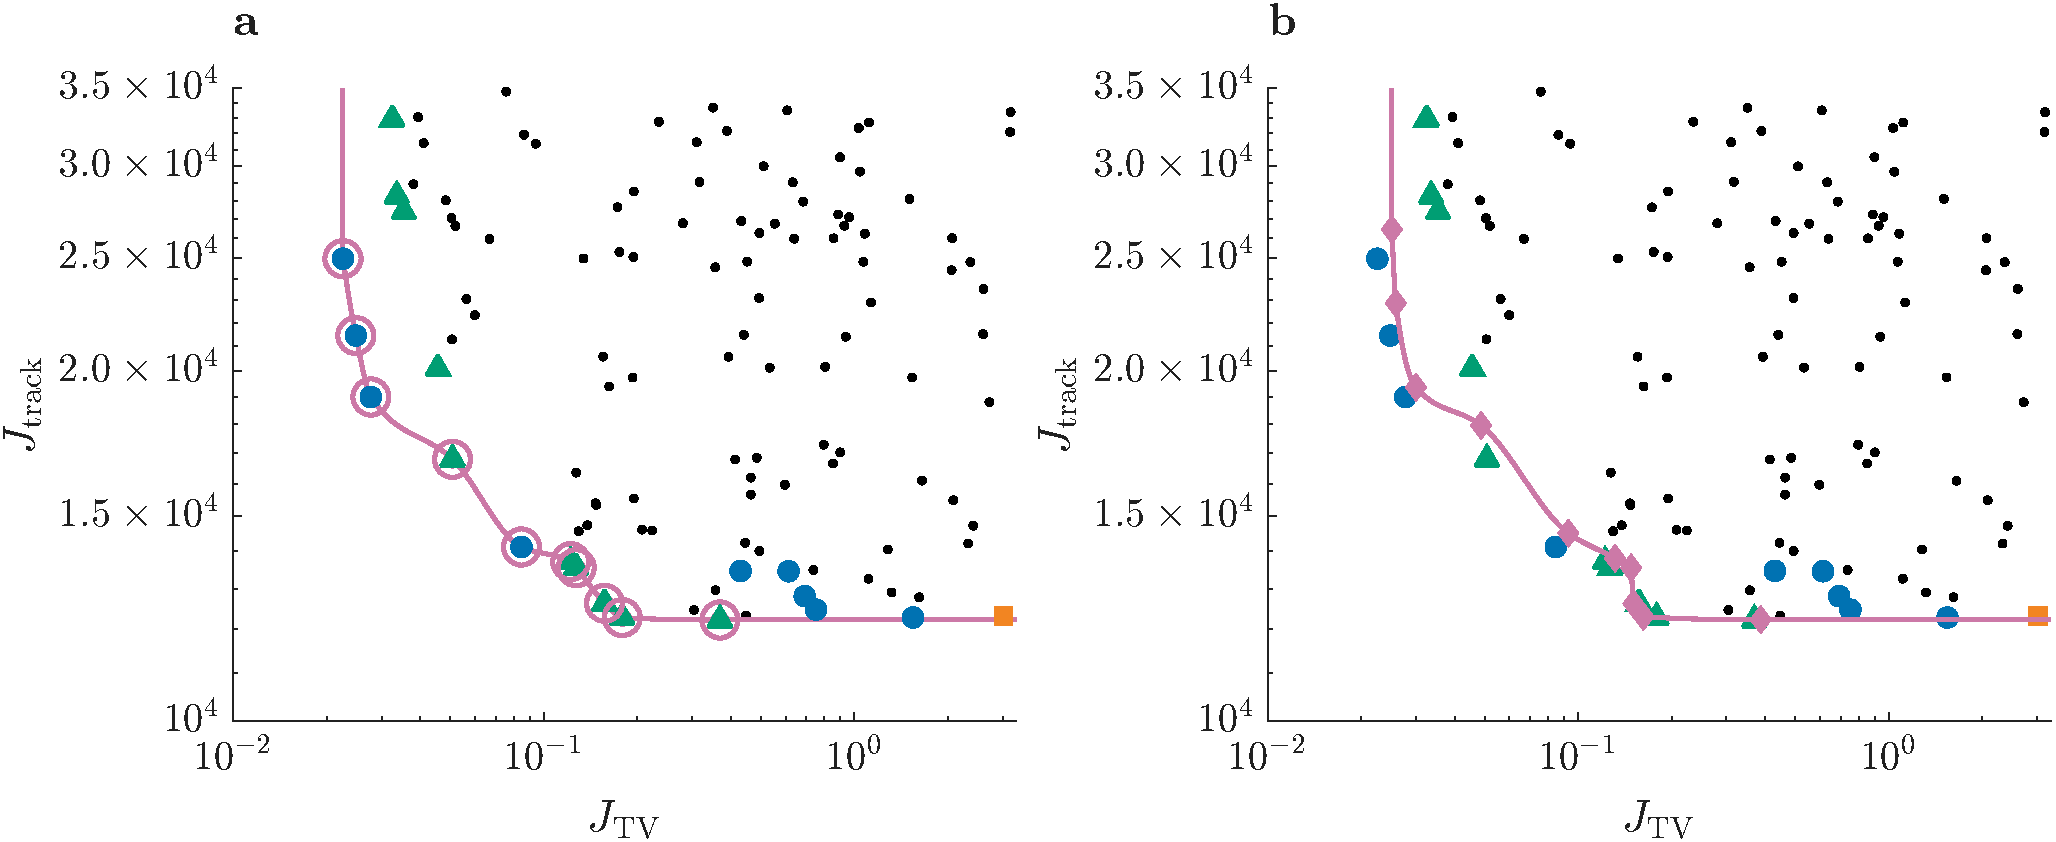
\includegraphics[width=0.95\linewidth]{refined_frontier_change.pdf}
\caption{Combined optimization frontier (left) and original/refined comparison (right). Refined-Pareto points are highlighted as purple diamonds; controllers promoted from non-Pareto to Pareto under full-fidelity refinement (with $z < 1$ in the original) are marked as black-edged stars.}
\label{fig:refined}
\end{figure}

Figure~\ref{fig:refined} compares the original optimization Pareto frontier (after DOE exclusion) against the refined frontier obtained by re-evaluating each controller at $f = 1$ with the same noise. The shape of the original frontier is largely preserved, but a small number of controllers that were dominated under truncated evaluation become Pareto-optimal under full fidelity. This is precisely the mismatch the multi-fidelity assumption forces one to confront: truncated evaluation is a useful ranker, but a handful of decisions near the frontier are sensitive to the extrapolation. The list of promoted controllers is exported to \texttt{results/txt~results/refined\_promoted\_frontier\_z\_lt\_1.txt}.

\subsection{Setpoint-schedule transferability}

\begin{figure}[!h]
\centering
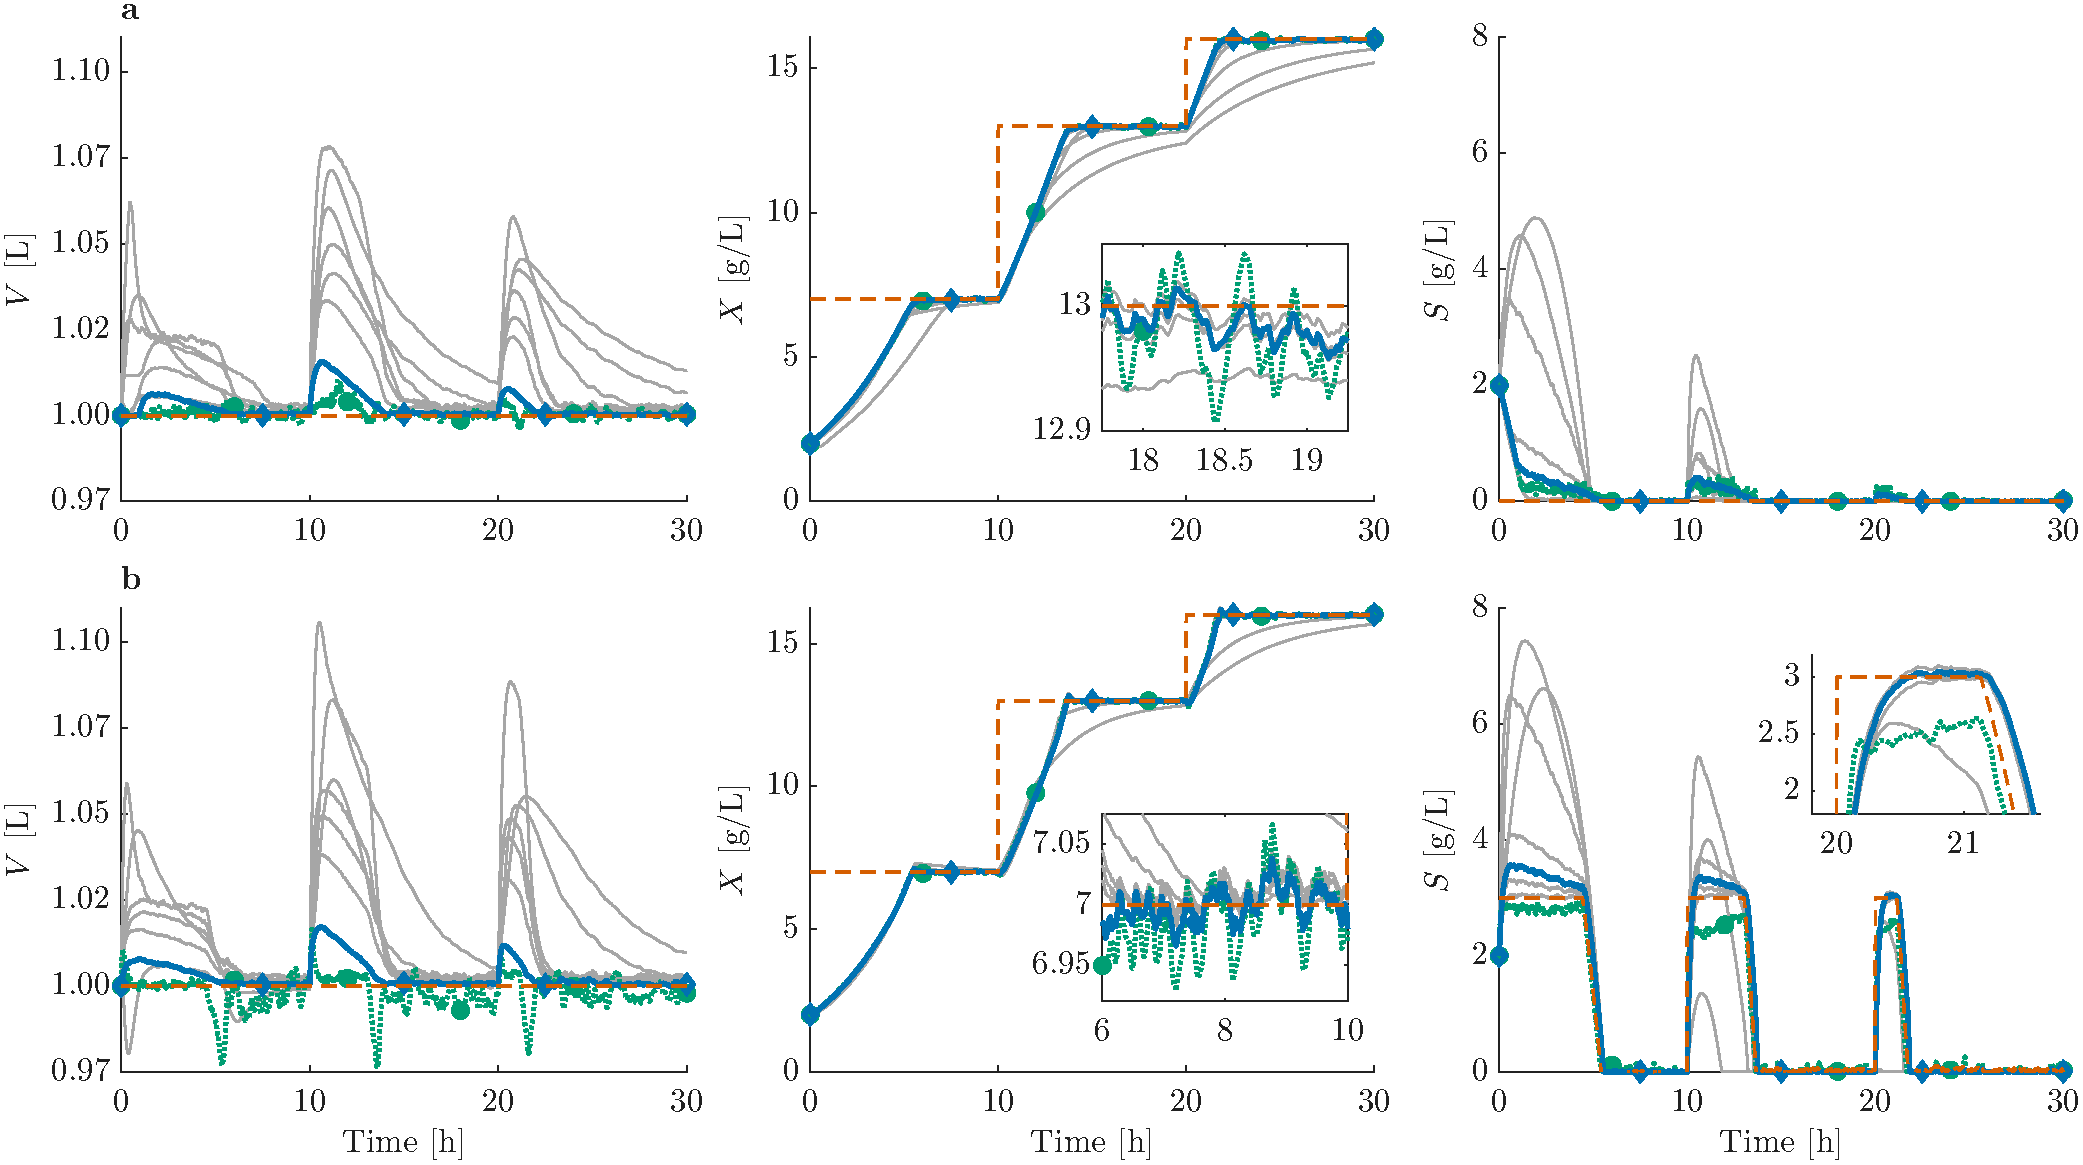
\includegraphics[width=0.95\linewidth]{setpoint_tracking.pdf}
\caption{Validation-scenario state trajectories across both simulation-scenario initial conditions and the three schedule segments ($X_{sp}: 7 \to 13 \to 16$). The deployment-selected controller is shown as a solid blue line with diamond markers, the benchmark as a dotted vermillion line with small circular markers, and all remaining non-selected Pareto controllers as thin neutral-grey solid lines. The setpoint trajectory is drawn as a dashed reference line. Markers are placed at uniformly spaced indices to aid identification without obscuring the curves.}
\label{fig:schedule_states}
\end{figure}

\begin{figure}[!h]
\centering
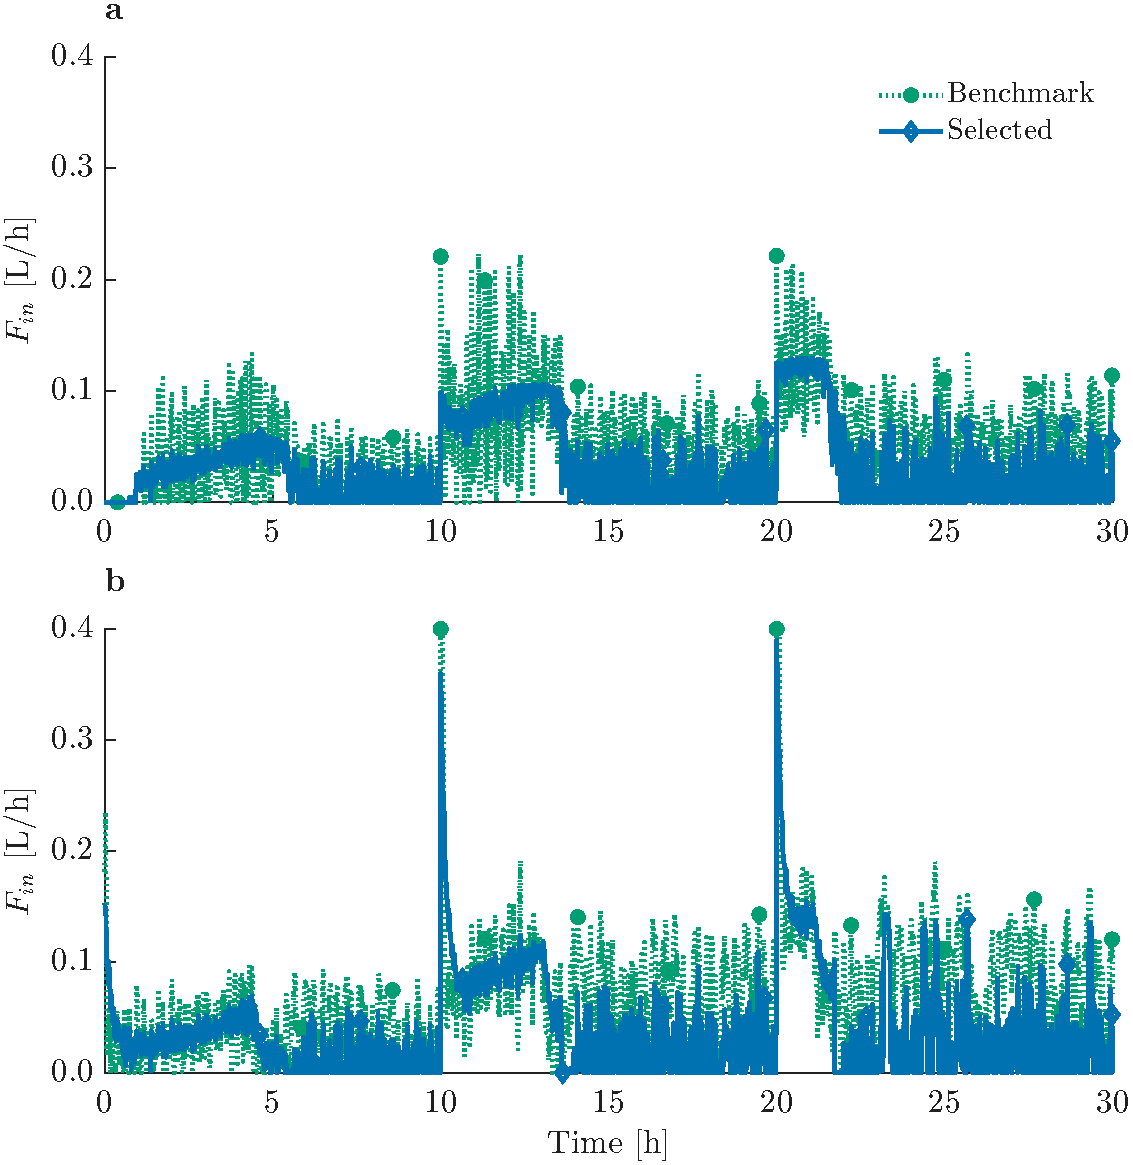
\includegraphics[width=0.85\linewidth]{setpoint_tracking_MV.pdf}
\caption{Manipulated-variable comparison on the validation scenario: $F_\mathrm{in}$ trajectory of the selected controller versus the benchmark, shown for both simulation-scenario initial conditions (subpanel \textbf{a}: scenario~1, subpanel \textbf{b}: scenario~2). The selected controller is plotted as a solid blue line with diamond markers placed at local maxima of its input profile, and the benchmark as a dotted vermillion line with small circular markers placed at local maxima and peak instants of its input profile. Markers are intended to highlight where each controller deviates most from a smooth setpoint-tracking response.}
\label{fig:schedule_MV}
\end{figure}

Figures~\ref{fig:schedule_states} and~\ref{fig:schedule_MV} provide the strongest external-validity evidence in the project. Several modified Pareto controllers outperform the benchmark across the multi-step schedule despite the BO never having trained on this scenario: they reach each new setpoint cleanly, settle within practically usable times, and use markedly less aggressive input motion. The selected controller in Figure~\ref{fig:schedule_states} achieves clean tracking on $V$ and $X$ across all three segments. Figure~\ref{fig:schedule_MV} explains \emph{why} it outperforms the benchmark on $\ssdu$: its $F_\mathrm{in}$ profile is smoother and less reactive than the benchmark's, while still responding to the setpoint changes at the expected instants.

The deployment-selection workflow documented in Section~\ref{sec:analysisscripts} matters here: the BO Pareto set serves as a curated shortlist for a human decision-maker. Once the optimization narrows the field to a handful of non-dominated candidates, picking the deployment controller is a small, transparent multi-criteria choice rather than another optimization problem. The selected controller (\texttt{ts\_20260211\_122653\_modified}) is the example of such a pick made on this codebase, motivated by simultaneous improvement in wall time, volume tracking, $\ssdu$, and biomass IAE, against a modest substrate-tracking sacrifice.

\subsection{Input-smoothing post-analysis}

\begin{figure}[!h]
\centering
\includegraphics[width=0.95\linewidth]{exploring_u_selected_controller_same_noise.pdf}
\caption{Original input $U$ (black) vs reduced-TV reconstruction $U^\star$ (coloured dashed) under the cumulative-sum constraint at nodes every $\SI{0.1}{h}$.}
\label{fig:explore_u}
\end{figure}

Figure~\ref{fig:explore_u} confirms that a substantial portion of the selected controller's high-frequency input activity can be removed without changing the cumulative input applied at each $\SI{0.1}{h}$ node. The reconstructed $U^\star$ preserves the same coarse trajectory but is visibly smoother. This suggests the BO-selected control trace contains structural slack --- there is room for a tighter $R_{\Delta u}$ penalty or a post-processing smoothing step without sacrificing the tracking trajectory.

\section{Discussion}
\label{sec:discussion}

Three threads run across the figures and reconcile into a single picture of how runtime-aware MFBO actually behaves on this problem.

The first concerns where the BO loop spends its budget. DOE absorbs roughly 59\% of the wall time, and the optimization phase shifts to candidates that are an order of magnitude cheaper per evaluation but retain mean fidelity $z \approx 0.81$. The lower bound on $z$ is governed by two distinct mechanisms. Physically, $z \cdot T = \SI{8.096}{h}$ coincides with the empirical settling timescale of the system (Section~5.5), so truncating significantly below this fidelity removes samples from a regime where many controllers are still in active transient. Statistically, the binding constraint is the $\jtv$ surrogate, whose 95\% extrapolation band contracts only slowly with $\tau$ (Section~5.6); the $\jtrack$ surrogate is much more stable but biased low. Because the $\jtv$ band contracts smoothly, small changes in $z$ around the current operating point should not change extrapolation quality abruptly, and a $\jtrack$-only objective would already admit operating fidelities $10$--$20\%$ below the present value. Online re-estimation of the surrogate (as discussed in Section~5.6) is the most direct path to reducing the bias on $\jtrack$ and, jointly with a better-conditioned surrogate model, to pushing the effective operating fidelity lower.

The second concerns the structure of the Pareto front. Case~1 and Case~2 specialize on opposite tails of the frontier in a way that is mechanistically tied to the NMPC horizon choices. Both runs collapse to $\Nc = 1$ on the Pareto set, but Case~1 frequently also picks $\Np = 1$, which reduces the controller to the LQR feedback law derived from~\eqref{eq:Plyap} applied to the nonlinear plant at the current state. This regime is naturally smooth (low $\jtv$) but slow (higher $\jtrack$). Case~2 retains $\Np > 1$, giving a single move that is anticipatory through the prediction window; the result is sharper tracking but larger move-to-move variation. The two runs are not contradictory; they are the two reachable sub-modes of an $\Nc = 1$ controller architecture, and the BO finite budget made each run commit to a different one. The benchmark sits strictly inside the Pareto set, achieving comparable $\sse$ to the best Case~2 controllers but with SSdU $8$ to $22\times$ larger --- it pays a large control-variation cost for no tracking advantage on this plant.

The third concerns deployment. Bi-objective optimization on $(\jtrack, \jtv)$ does not guarantee state-wise settling, and the substrate ($S$) settling rate is the bottleneck (Section~5.5). The refined-frontier figure (Section~5.7) shows that a small subset of the optimization-phase Pareto rank ordering changes under full-fidelity replay, so the deployment recommendation should not be read directly off the BO surrogate. Instead, the workflow shown in Sections~\ref{sec:analysisscripts} and~5.8 --- BO narrows the field to a small Pareto set, full-fidelity replay validates that ranking, and a human picks among a handful of candidates using a small set of practical metrics --- is the correct decision pipeline. The setpoint-schedule transferability evidence is positive: several Pareto controllers beat the benchmark on a scenario the BO never saw, suggesting that the BO-Pareto-then-engineer workflow is robust to regimes outside the optimization scenario.

\section{Conclusion}
\label{sec:conclusion}

The \texttt{MFBO\_NMPC} codebase implements a runtime-aware multi-fidelity Bayesian-optimization workflow for bi-objective NMPC tuning that operates correctly on a reduced bioprocess dilution plant. The DOE phase is the dominant cost, the optimization phase shifts to cheaper candidates while retaining high mean fidelity, and the recovered Pareto front has a robust knee that overlaps cleanly between two independent runs. The Chebyshev fraction surrogate is an excellent ranker ($R^2 = 0.992$ for $\jtv$, $0.9998$ for $\jtrack$, $98.76\%$ of files within 1\% endpoint error), but its 95\% extrapolation band is asymmetric across the two objectives: the $\jtrack$ surrogate is biased low but tight, while the $\jtv$ surrogate contracts more slowly and is the binding constraint on lowering the operating fidelity. Both observations point to the same remedy: a low-parameter, monotone, regularized surrogate that enforces $\phi(0) = 0$ and $\phi(1) = 1$, ideally re-estimated online during the BO run, would correct the $\jtrack$ bias and tighten the $\jtv$ band.

The two BO runs specialize on opposite tails of the Pareto front in a way that is mechanistically explained by the choice of $\Np$: the low-$\jtv$ tail is the LQR-collapsed $\Nc = \Np = 1$ regime, while the low-$\jtrack$ region is the $\Nc = 1, \Np > 1$ anticipatory regime. The benchmark sits strictly inside this front. The setpoint-schedule analysis demonstrates that the BO-Pareto-then-engineer workflow transfers to scenarios outside the optimization regime. State-wise settling is the principal gap: minimizing $(\jtrack, \jtv)$ does not guarantee balanced settling across outputs, particularly for substrate, and a tighter settling-aware objective formulation is the recommended next iteration.

\end{document}
